First, we will go over the handshake that TLS 1.2 and prior versions used. In this example the server uses a certificate to prove its identity to the client, but the client does not use a certificate.
\\\\
This illustration shows the entire handshake process, including the TCP handshake, which is not directly part of the TLS handshake, but still contributes to TLS latency. 

\begin{figure}[H]
    \centering
    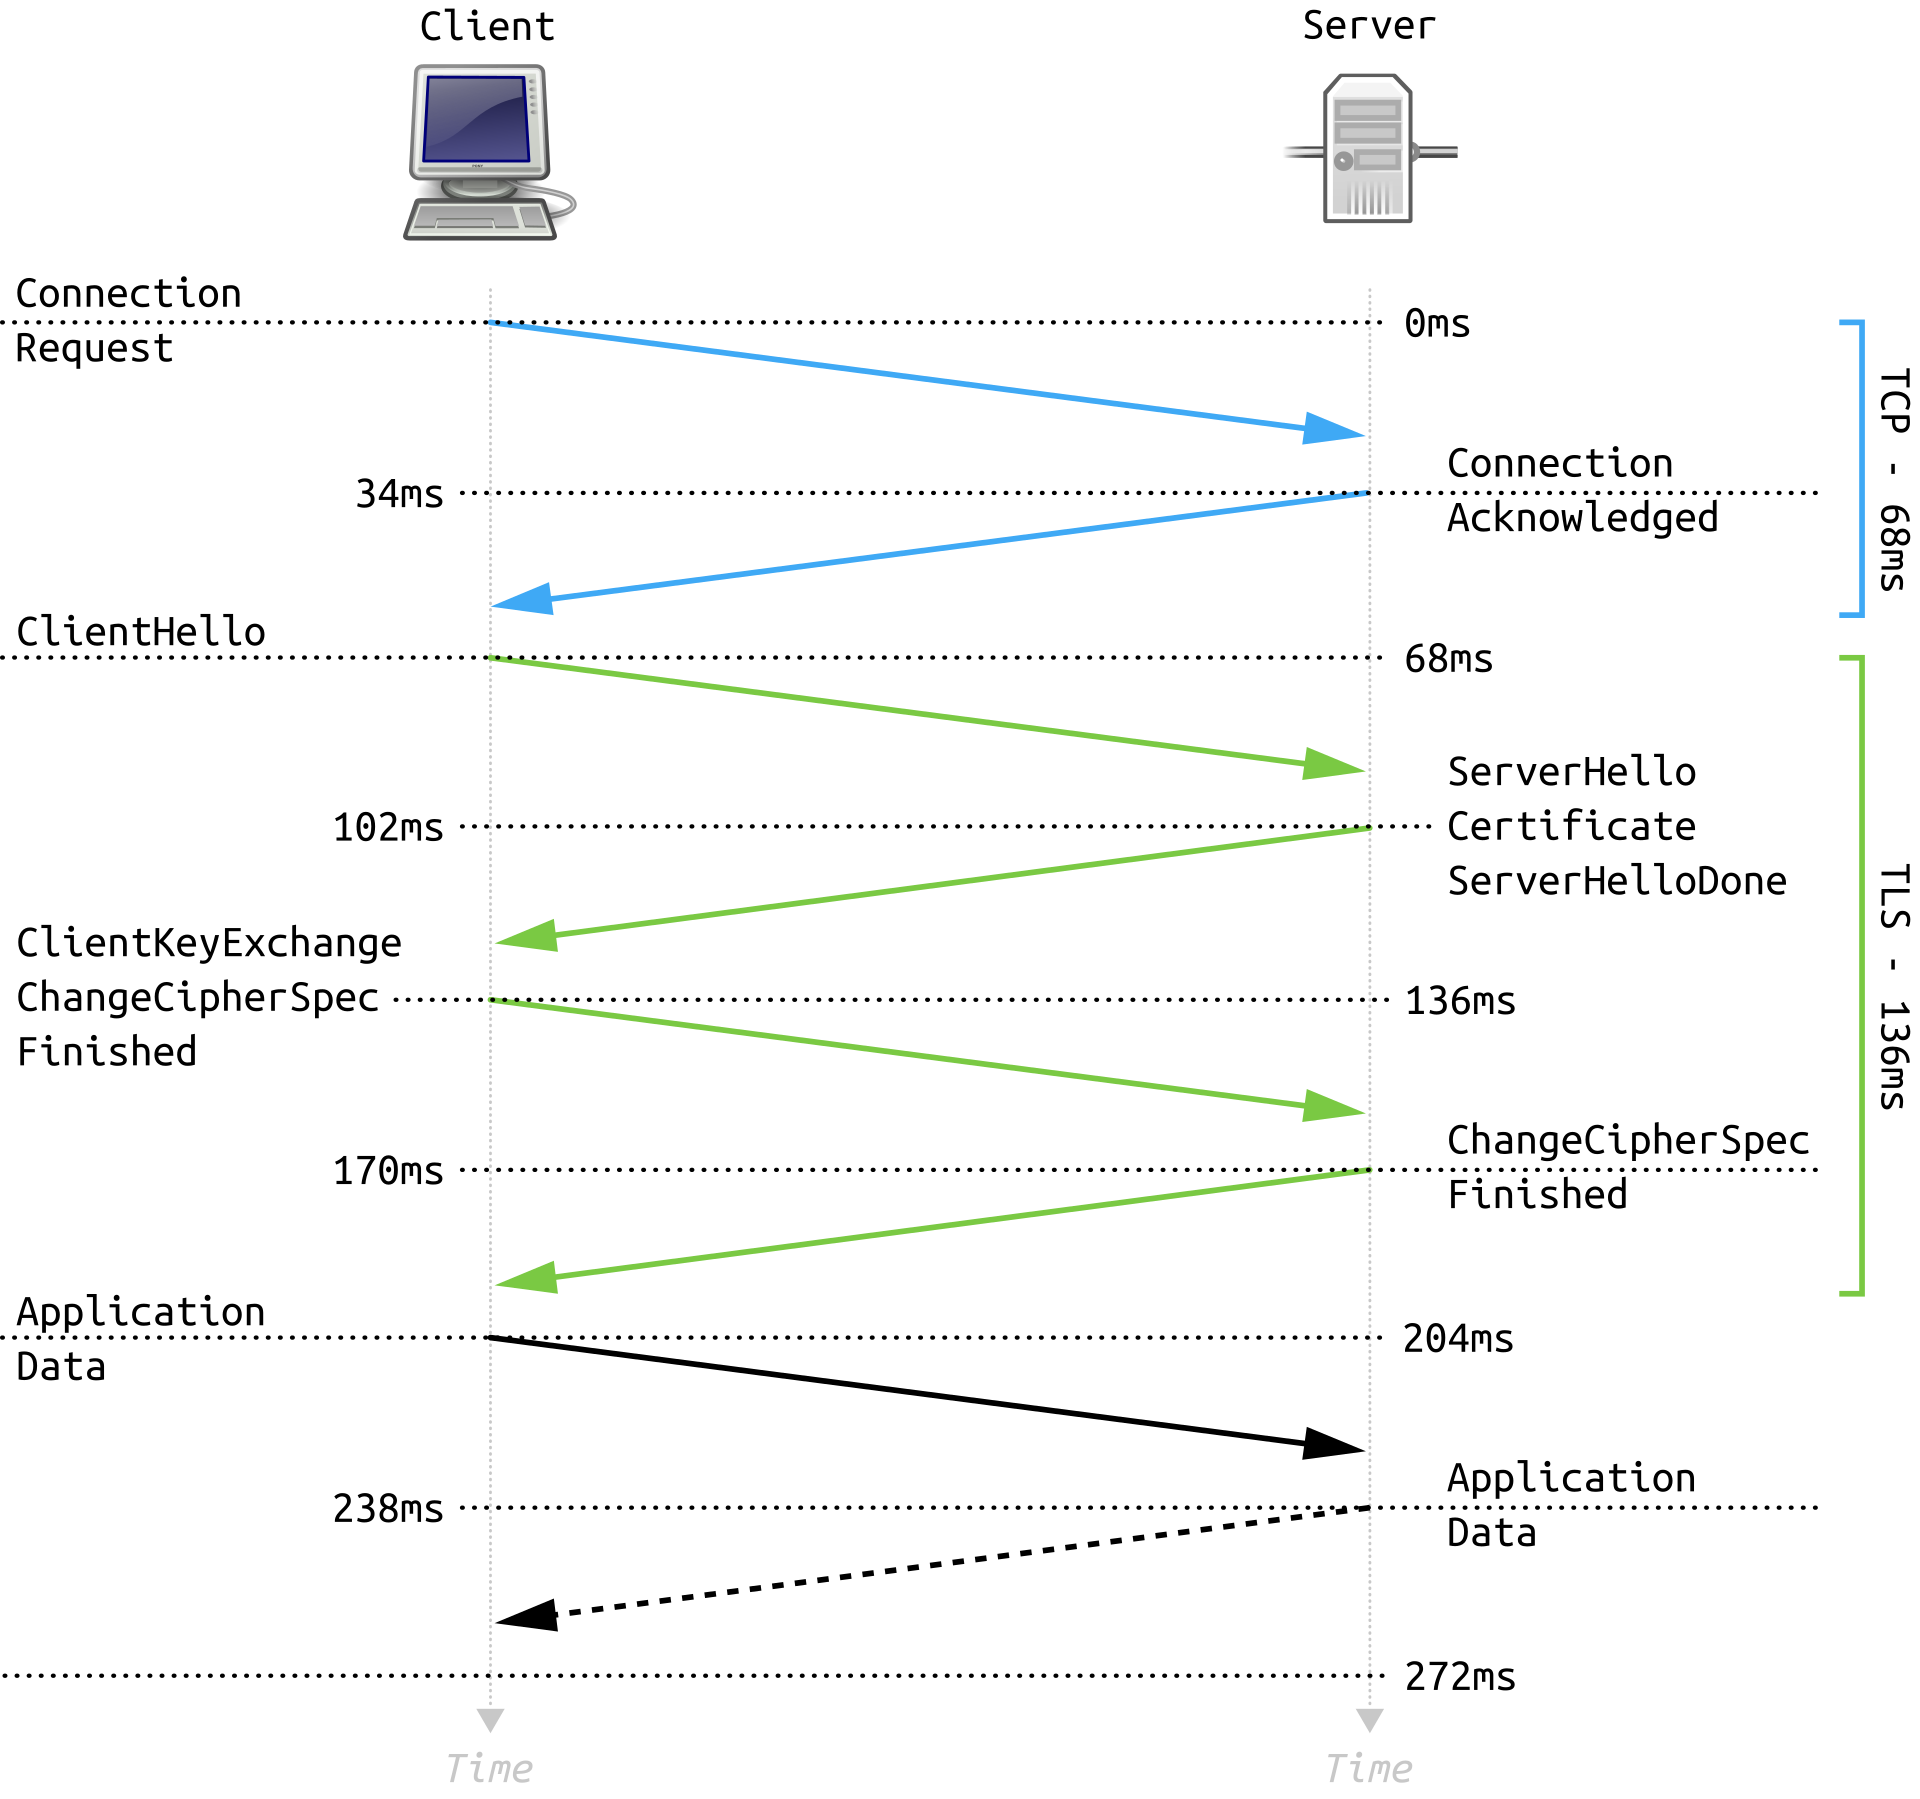
\includegraphics[width=0.8\textwidth]{Figures/Full_TLS_1_2_Handshake.png}
    \caption{TLS 1.2 Handshake}
    \label{fig:tls_handshake}
\end{figure}

The handshake can be separated into four phases:
\begin{enumerate}
    \item Negotiation: The client starts the handshake by sending a \texttt{ClientHello} message. The message contains the client's supported TLS versions, a list of supported ciphers, a random number and suggested compression methods.
    \\\\
    The server responds with a \texttt{ServerHello} message. The message contains the chosen TLS version, a chosen cipher, a random number and a chosen compression method from the supported ones the client sent before.
    \\
    The server also sends its certificate, which contains the server's public key.
    \\
    If the key exchange methode is a version of Diffie Hellman, the server will also send a \texttt{ServerKeyExchange} message.
    \\
    The server also sends a \texttt{ServerHelloDone} message, which signals that the server is done with the negotiation phase.
    \\\\
    The client then sends a \texttt{ClientKeyExchange} message, which, depending on cipher used, contains the pre-master secret encrypted by the public key of the server, public key, or nothing.
    \\\\
    The server and client then compute a common secret using the random numbers they shared and the pre-master secret. The common secret is also called master secret and is used to derive all other keys, like the session key or MAC key.
    \\
    \item The Clients sends a \texttt{ChangeCipherSpec} message, which signals that the client will start using the negotiated cipher and compression method.
    \\
    The client sends a encrypted \texttt{Finished} message, which contains a hash of all previous messages. The server will then try to decrypt the message and check if the hash is correct. If the hash is not correct the handshake failed.
    \\
    \item The server sends a \texttt{ChangeCipherSpec} message. The process is the same as in the client phase, just with the roles reversed.
    \\
    \item Application phase: The handshake is complete and the server and client can now send application data.
\end{enumerate}

This handshake requires 2 round trips, not including the TCP handshake, which causes quite a bit of latency before the client and server can start exchanging application data.
\\\\
The handshake for TLS 1.3 removes 1 round trip most of the time. Compared to the TLS 1.2 handshake the client includes guesses for which key exchange methode the server will use and the public keys for the gussed key exchange methods in the \texttt{ClientHello} message. If one of the guesses matches the server, it allows the server to send the \texttt{ServerHello}, Certificate and \texttt{Finished} message, without having to wait for a client response.
\\
TLS 1.3 also includes support for a 0 round trip data handshake. When the client and server have a pre shared key the client can include data in the first flight of data by appending it to the 1-RTT handshake.
\\\\
Because the key exchange is compute heavy, TLS offers a way to resume a session using session IDs. For this the client remembers the session ID and assiocates it with the IP and port combination of the server. When rebuidling the connection the client sends the session ID in the \texttt{ClientHello} message. The server then looks up the session ID and if it finds it, it can skip the key exchange and go straight to the application phase. This removes the need for the key exchange. Both sides must have the same master secret, preventing eavesdropping on the session ID. 
\\
Sessions can also be used for SSO, as it guranatees that the client is the same as the one that established the session.
\\\\
Another way to restore sessions is using session tickets. The server sends a session ticket to the client for storing. The client then sends the session ticket in the \texttt{ClientHello} message. The server then decrypts the session ticket and can skip the key exchange. Session tickets allow the server to forget the session while still being able to resume it with the client later.
\\\\
QUIC is able to do the entire handshake in just 1 roundtrip by using UDP instead of TCP and including the TLS handshake in the first messages. QUIC then uses its own flow control to ensure that all messages are delivered in order. Because QUIC is not the topic of this paper, we will not go into more detail about it.